% !TEX root = handbook-physics.tex
%!TEX TS-program = pdflatex
%!TEX encoding = UTF-8 Unicode


\chapter{Work And Mechanical Energy}
\label{ch-03}
\zhtitle{功与机械能}

\section{Energy, Work and Power}
\label{sec-3.1}
\zhtitle{能量、功与功率}
\subsection{}\label{3.1.1} Energy is a scalar physical quantity, which is a common measure of the various forms of motion of matter dealt with in physics. The energy of a system quantitatively characterizes this system with respect to the conversions of motion that are possible within it. These conversions take place due to the in­teraction between parts of the system, both with one another and with external bodies (the environment). The concept of various forms of energy has been introduced in physics to ana­lyze the qualitatively different forms of motion and the interac­tions corresponding to them. These include: mechanical \ssect{3.4.1}, internal \ssect{9.1.2}, electromagnetic \ssect{31.2.1}, nuclear \ssect{42.2.2} and various other forms of energy.
\zhpar{能量是标量物理量，是物理学中用来度量物质各种运动形式的共同量度。系统的能量定量地刻画了该系统内各种运动形式之间可能发生的转化。这些转化是由系统各部分之间的相互作用（彼此之间的相互作用以及与外部物体（环境）之间的相互作用）引起的。物理学中引入各种形式的能量概念，用以分析性质不同的运动形式及与之对应的相互作用。这些形式包括：机械能 \ssect{3.4.1}、内能 \ssect{9.1.2}、电磁能 \ssect{31.2.1}、核能 \ssect{42.2.2} 以及其他各种形式的能量。}

\subsection{}\label{3.1.2} The mechanical motion of a body is changed by forces exerted on the body by other bodies. Used in mechanics for a
quantitative description of such a process of energy exchange between interacting bodies is the concept of the work done by the forces applied to the body being considered. An \redem{element of work} done by force $\vb{F}$ in the infinitely small displacement $d\vb{r}$ is the scalar quantity
\zhpar{物体的机械运动会因其他物体施加于该物体的力而改变。力学中用来定量描述相互作用物体之间这种能量交换过程的概念，是作用于所考虑物体上的力所做的功。力 $\vb{F}$ 在无限小位移 $d\vb{r}$ 中所做的\redem{元功}是一个标量，其表达式如下式所示。}
\begin{equation*}%
\var{W}= \vb{F}\,\dd\vb{r}= \vb{Fv}\dd{t},
\end{equation*}
where $\vb{r}$ and $\vb{v} = \dv*{\vb{r}}{t}$ are the radius vector and velocity of the point of the body at which the force is applied, and $\dd t$ is the infinitely short time interval during which force $\vb{F}$ performs the work $\var{W}$ (the meaning of the notation $\var{W}$ is given in \ssect{3.1.8}). In rectangular Cartesian coordinates
\zhpar{式中 $\vb{r}$ 与 $\vb{v} = \dv*{\vb{r}}{t}$ 分别为力作用点的位矢和速度，$\dd t$ 为力 $\vb{F}$ 做功 $\var{W}$ 所经历的无限短的时间间隔（符号 $\var{W}$ 的含义见 \ssect{3.1.8}）。在直角笛卡儿坐标系中，元功的表达式如下。}
\begin{align*}%
\var{W} & = F_{x}\dd x + F_{y}\dd y + F_{z}\dd z, \\
&  = (F_{x}v_{x}+ F_{y}v_{y} + F_{z}v_{z}) \dd t,
\end{align*}
where $x$, $y$ and $z$ are the coordinates of the point of application of the force, and $F_{x}$, $F_{y}$, $F_{z}$ and $v_{x}$, $v_{y}$, $v_{z}$ are the projections of vectors $\vb{F}$ and $\vb{v}$ on the coordinate axes.
\zhpar{式中 $x$、$y$、$z$ 为力作用点的坐标，$F_{x}$、$F_{y}$、$F_{z}$ 以及 $v_{x}$、$v_{y}$、$v_{z}$ 分别为矢量 $\vb{F}$ 与 $\vb{v}$ 在各坐标轴上的投影。}

\subsection{}\label{3.1.3} The expression for an element of work can also be pre­sented in the form
\zhpar{元功的表达式也可以写成如下形式。}
\begin{equation*}%
\var{W} = F \, \dd s \cos \alpha = F_{\tau} \dd s,
\end{equation*}
where $\dd s = \abs{\dd \vb{r}}$ is an element of the length of the path of the point of force application during the infinitely short time interval $\dd t$, $\alpha$ is the angle between vectors $\vb{F}$ and $\dd \vb{r}$, and $F_{\tau} = F \cos \alpha$ is the projection of the force in the direction of the displacement $\dd \vb{r}$. A force normal to the path of its point of appli­cation performs no work.
\zhpar{式中 $\dd s = \abs{\dd \vb{r}}$ 为力作用点在无限短时间间隔 $\dd t$ 内所经路径的弧长元，$\alpha$ 为矢量 $\vb{F}$ 与 $\dd \vb{r}$ 之间的夹角，$F_{\tau} = F \cos \alpha$ 为力在位移 $\dd \vb{r}$ 方向上的投影。与受力作用点所经路径相垂直的力不做功。}

Force $\vb{F}$ is called the \redem{motive force} if $F_{\tau} >0$, so that $\var{W} > 0$. If $F_{\tau} < 0$ (so that $\var{W} < 0$), force $\vb{F}$ is called the \redem{retarding force} (\redem{force of resistance}).
\zhpar{若 $F_{\tau} >0$，从而 $\var{W} > 0$，则力 $\vb{F}$ 称为\redem{驱动力}。若 $F_{\tau} < 0$（从而 $\var{W} < 0$），则力 $\vb{F}$ 称为\redem{阻滞力}（即\redem{阻力}）。}

\subsection{}\label{3.1.4} If a mechanical system is subject to the simultaneous action of forces $ \vb{F}_{1},\,\vb{F}_{2}\, \ldots \,\vb{F}_{n}$, the work $\var{W}$ done by them during the infinitely short time $\dd t$ is equal to the algebraic sum of the work done during the same time $\dd t$ by each of the forces separately. Thus
\zhpar{若机械系统同时受到力 $\vb{F}_{1},\,\vb{F}_{2}\, \ldots \,\vb{F}_{n}$ 的作用，则在无限短时间 $\dd t$ 内它们所做的总功 $\var{W}$ 等于各力在同一时间 $\dd t$ 内分别做功的代数和。因此有如下关系式。}
\begin{equation*}%
\var{W} = \sum_{i=1}^{n} \var{W}_{i} = \sum_{i=1}^{n} \vb{F}_{i} \dd \vb{r}_{i} = \sum_{i=1}^{n} \vb{F}_{i}\vb{v}_{i} \dd t,
\end{equation*}
where $\vb{r}_{i}$ and $\vb{v}_{i}$ are the radius vector and velocity of the point of application of force $\vb{F}_{i}$.
\zhpar{式中 $\vb{r}_{i}$ 与 $\vb{v}_{i}$ 分别为力 $\vb{F}_{i}$ 作用点的位矢和速度。}

For example, for a particle $\vb{r}_{i} = \vb{r}$ is the radius vector of the particle and $\vb{v}_{i} = \vb{v}$ is its velocity. Accordingly, $\var{W} = \vb{F} \dd \vb{r} = \vb{Fv}\dd t$, where $\vb{F} = \sum_{i=1}^{n} \vb{F}_{i}$ is the resultant force \ssect{2.2.2}. It follows from Newton's second law \ssect{2.4.1} that for a particle
\zhpar{例如，对于质点，$\vb{r}_{i} = \vb{r}$ 为质点的位矢，$\vb{v}_{i} = \vb{v}$ 为其速度。相应地，$\var{W} = \vb{F} \dd \vb{r} = \vb{Fv}\dd t$，其中 $\vb{F} = \sum_{i=1}^{n} \vb{F}_{i}$ 为合力（见 \ssect{2.2.2}）。由牛顿第二定律（见 \ssect{2.4.1}）可知，对质点有如下关系式。}
\begin{equation*}%
\var{W}= \vb{v} \dd \vb{p},
\end{equation*}
where $\vb{p} = m \vb{v}$ is the momentum of the particle, and $m$ is its mass.
\zhpar{式中 $\vb{p} = m \vb{v}$ 为质点的动量，$m$ 为其质量。}

In the translational motion of a perfectly rigid body $\dd \vb{r}_{i} = = \dd \vb{r}_{C}$ and $\vb{v}_{i} = \vb{v}_{C}$, where $\vb{r}_{C}$ and $\vb{v}_{C}$ are the radius vector and velocity of the centre of mass \ssect{2.3.3} of the body.
\zhpar{对于绝对刚体的平动，$\dd \vb{r}_{i} = = \dd \vb{r}_{C}$，$\vb{v}_{i} = \vb{v}_{C}$，其中 $\vb{r}_{C}$ 与 $\vb{v}_{C}$ 分别为物体质心（见 \ssect{2.3.3}）的位矢和速度。}

The work done by internal forces in any motion of a perfectly rigid body equals zero. Hence, in the translational motion of such a body $\var{W} = \vb{F}^{\textrm{ext}} \dd \vb{r}_{C} = \vb{F}^{\textrm{ext}}\vb{v}_{C} \dd t$, where $\vb{F}^{\textrm{ext}}$ is the principal vector of external forces \ssect{2.5.2}. It follows from the law of motion of the centre of mass \ssect{2.5.3} that
\zhpar{任意运动中绝对刚体内力所做的功都等于零。因此，在这种物体的平动中，$\var{W} = \vb{F}^{\textrm{ext}} \dd \vb{r}_{C} = \vb{F}^{\textrm{ext}}\vb{v}_{C} \dd t$，其中 $\vb{F}^{\textrm{ext}}$ 为外力的主矢（见 \ssect{2.5.2}）。由质心运动定律（见 \ssect{2.5.3}）可得如下关系式。}
\begin{equation*}%
\var{W} = \vb{v}_{C} \dd \vb{p},
\end{equation*}
where $\vb{p} = m\vb{v}_{C}$ is the momentum of a rigid body of mass $m$ travelling at the velocity $\vb{v} = \vb{v}_{C}$.
\zhpar{式中 $\vb{p} = m\vb{v}_{C}$ 为质量为 $m$、以速度 $\vb{v} = \vb{v}_{C}$ 作平动的刚体的动量。}


\subsection{}\label{3.1.5} The work $W$ done by force $\vb{F}$ along a finite portion of the path $L$ of its point of application is equal to the algebraic sum of the work done over all the infinitely small portions of this path, i.e. it is expressed by the line integral
\zhpar{力 $\vb{F}$ 沿作用点路径 $L$ 的有限段所做的功 $W$，等于该段路径上所有无限小段内所做功的代数和，即可用如下线积分表示。}
\begin{equation*}%
W = \int_{(L)} \vb{F} \dd \vb{r} = \int_{0}^{s} F_{\tau} \dd s,
\end{equation*}
where $s$ is the length of arc measured off along the path from the beginning of the portion of the path being considered, and $F_{\tau}$ the projection of the force onto the direction of displace­ment $\dd \vb{r}$ of the point of force application. 
\zhpar{式中 $s$ 为从所考虑路径段起点沿路径量取的弧长，$F_{\tau}$ 为力在力作用点位移 $\dd \vb{r}$ 方向上的投影。}
\begin{marginfigure}%[!ht]
%\begin{wrapfigure}{r}{0.5\linewidth}
\centering
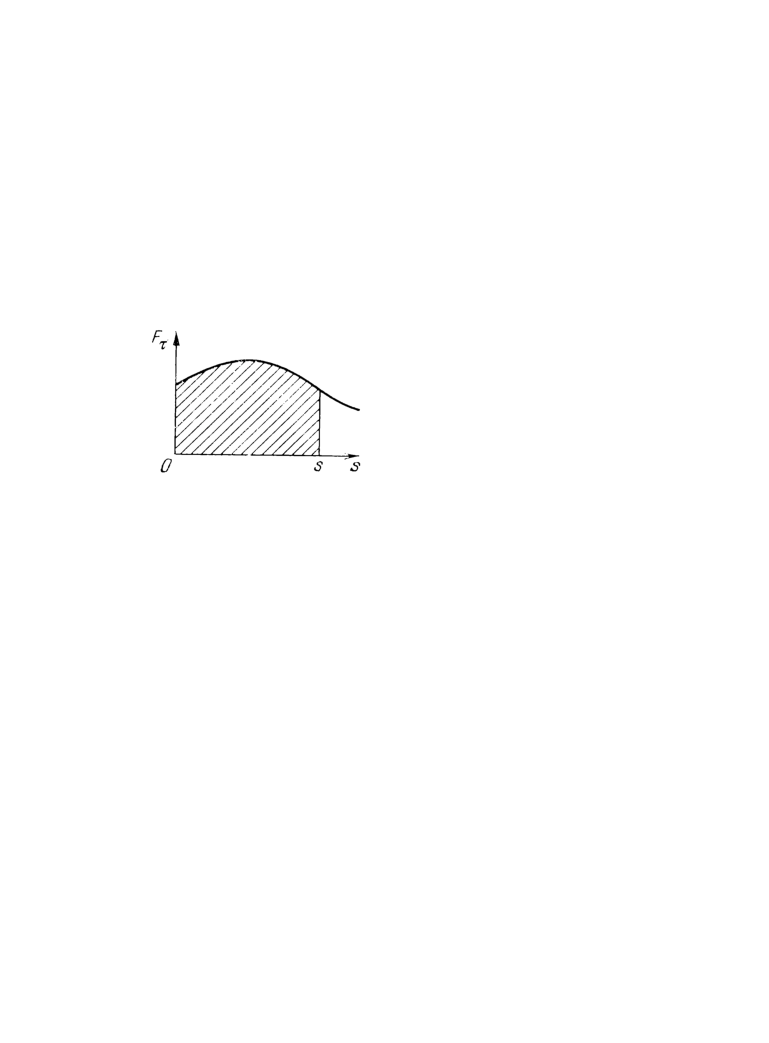
\includegraphics[width=0.8\textwidth]{figs/ch-03/fig-03-01.pdf}
%\input{figs/ch-03/fig-03-01}
%  \vspace{-13pt}
\sidecaption{Graphical representation of the resultant work.\zhcap{合力做功的图形表示。}\label{fig-03-01}}
\end{marginfigure}


To calculate this integral it is necessary to know the dependence of $F_{\tau}$ on $s$ along the given path $L$. If this dependence is represented graphically (\figr{fig-03-01}), the required work $W$ is proportional to the hatched area in \figr{fig-03-01}.
\zhpar{要计算该积分，需要知道沿给定路径 $L$ 时 $F_{\tau}$ 与 $s$ 的依赖关系。若将此关系用图线表示（见 \figr{fig-03-01}），则所求功 $W$ 与 \figr{fig-03-01} 中阴影面积成正比。}


\subsection{}\label{3.1.6} \redem{Potential-field (conservative)} forces are ones whose work depends only on the initial and final positions of their points of application; it depends neither on the shape of the path of these points nor on their laws of motion along this path.
\zhpar{\redem{有势（保守）力}是指做功仅取决于其作用点的初始与终了位置的力；它既与作用点所经路径的形状无关，也与作用点沿该路径的运动规律无关。}

For example, the forces of interaction between the parts (i.e. particles) of a system are said to be potential (conservative) forces if they depend only upon the configuration of the system, i.e. on the relative position of all its particles. The work done by these forces in moving the system from one arbitrary position to another is independent of the kind of displacement, but is completely determined by the initial and final configurations of the system. Examples are the forces of electrostatic and grav­itational interaction.
\zhpar{例如，若系统各部分（即质点）之间的相互作用力仅取决于系统的位形，即仅取决于系统所有质点的相对位置，则称这些力为有势（保守）力。这些力使系统从任一位形移动到另一位形时所做的功与位移的方式无关，完全由系统的初始和终了位形决定。静电相互作用力与引力相互作用都是这类力的例子。}

\begin{marginfigure}%[!ht]
%\begin{wrapfigure}{r}{0.5\linewidth}
\centering
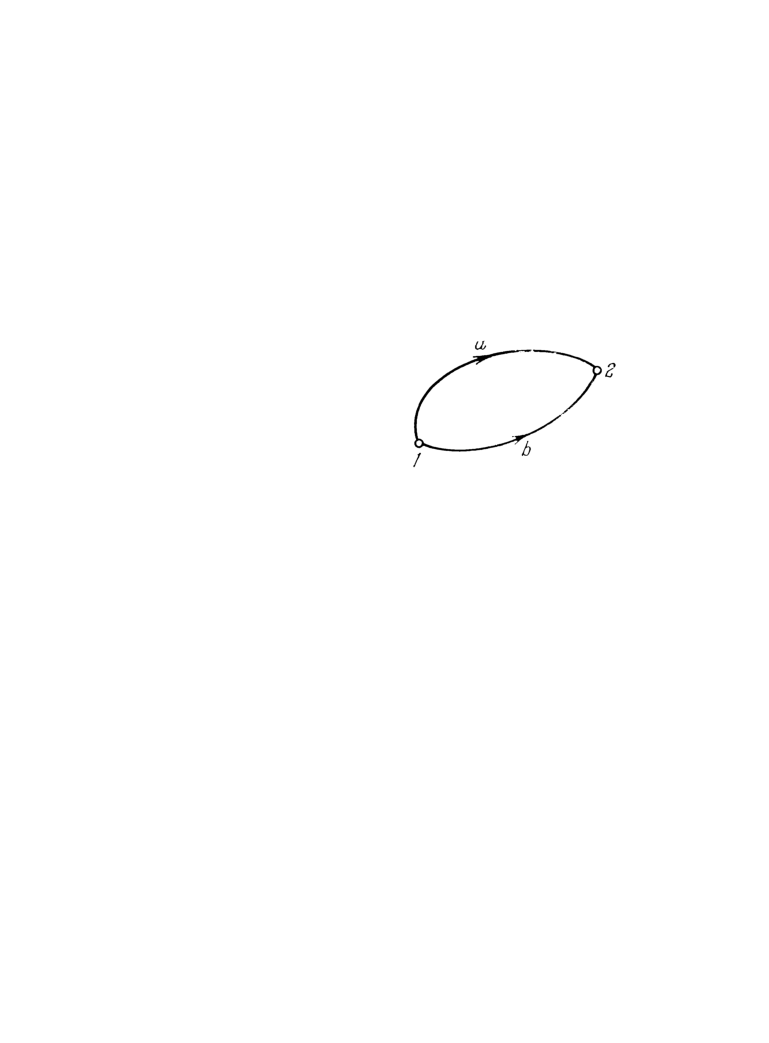
\includegraphics[width=0.8\textwidth]{figs/ch-03/fig-03-02.pdf}
%\input{figs/ch-03/fig-03-01}
%  \vspace{-13pt}
\sidecaption{Graphical representation of the resultant work.\zhcap{合力做功的图形表示。}
\label{fig-03-02}}
\end{marginfigure}

A \redem{steady (stationary)} field \ssect{2.2.1} is said to be \redem{potential}, or con­servative, if force $F$, which it exerts on a particle located in the field, is a potential, or conservative force. This implies that force $F$ depends only upon the position of the particle in the field, and that the amounts of work done by force $F$ in displacing the particle from one arbitrary position (1) to ano­ther (2) (\figr{fig-03-02}) along any two paths, for instance, $1a2$ (work
$W_{1a2}$) and $1b2$ (work $W_{1b2}$), are the same:
\zhpar{稳定（定常）场（见 \ssect{2.2.1}）称为\redem{有势场}或保守场，如果场作用于位于场中某质点的力 $F$ 是有势力或保守力。这意味着力 $F$ 仅依赖于质点在场中的位置，并且力 $F$ 使质点从任一位置（1）移动到另一位置（2）（见 \figr{fig-03-02}）时，沿任意两条路径（例如 $1a2$（所做功为 $W_{1a2}$）与 $1b2$（所做功为 $W_{1b2}$））所做的功相等：}
\begin{equation*}%
W_{1a2} = W_{1b2} = \int_{1}^{2} \vb{F} \dv{\vb{r}} .
\end{equation*}
Accordingly, the work done by a conservative force in displac­ing its point of application along any closed path $L$ (for exam­ple, $1a2b1$) is equal to zero:
\zhpar{因此，保守力使其作用点沿任意闭合路径 $L$（例如 $1a2b1$）移动时所做的功等于零，即下式成立。}
\begin{equation*}%
\oint_{(L)} \vb{F} \dd{\vb{r}} \equiv 0.
\end{equation*}
In the general case, the external bodies that set up the field being considered can be in motion with respect to an inertial frame of reference, so that their field is not stationary, i.e. force $\vb{F}$ depends explicitly on time: 
\zhpar{一般地，产生所考虑场的外部物体相对于惯性参考系可能在运动，此时场不是稳定的，即力 $\vb{F}$ 显式地依赖于时间，如下式所示。}
\begin{equation*}%
\pdv{\vb{F}}{t} \nequiv 0.
\end{equation*}
A \redem{nonstationary field} is a \redem{conservative} one if the work done by force $\vb{F}$ upon instanta­neous displacement of its point of application along any closed path $L$ equals zero:
\zhpar{若非稳定场中力 $\vb{F}$ 使其作用点沿任意闭合路径 $L$ 做瞬时位移时所做的功等于零，则该\redem{非稳定场}是\redem{保守的}，即下式成立。}
\begin{equation*}%
\oint_{(L)} \vb{F} \dd{\vb{r}} \equiv 0.
\end{equation*}
Here $\vb{F}$ depends, not only on the coordinates of the point of appli­cation, but on the time as well. To calculate this integral, how­ ever, time is assumed to be a fixed parameter.
\zhpar{这里 $\vb{F}$ 不仅依赖于作用点的坐标，还依赖于时间。但是，计算该积分时，时间被视为固定参数。}


\subsection{}\label{3.1.7} Among the nonconservative forces are dissipative and gyroscopic forces. \redem{Dissipative forces} are ones whose total work done in displacing a closed system in any way is always negative. Such, for instance, are the forces of sliding friction and the forces retarding the motion of bodies in liquids and gases. In contrast to conservative forces, dissipative forces depend, not only on the relative positions of the interacting bodies, but on their relative velocities as well.
\zhpar{非保守力包括耗散力与陀螺力。\redem{耗散力}是指在任意方式下使封闭系统产生位移时，其所做总功始终为负的力。例如滑动摩擦力，以及阻碍物体在液体和气体中运动的力，都属于耗散力。与保守力不同，耗散力不仅取决于相互作用物体之间的相对位置，还取决于它们的相对速度。}

\redem{Gyroscopic forces} are ones that depend upon the velocity of the particle on which they act. They are directed perpendicular to this velocity. An example is the Lorentz force \ssect{24.1.1} exerted by a magnetic field on a charged particle travelling in this field. The work done by gyroscopic forces is always equal to zero, regardless of how the particle is displaced.
\zhpar{\redem{陀螺力}是指依赖于其所作用质点速度的力，其方向与该速度垂直。例如，磁场作用于在其中运动的带电粒子上的洛伦兹力（见 \ssect{24.1.1}）就是一种陀螺力。陀螺力所做的功总等于零，与质点如何位移无关。}

A mechanical system (system of particles) is said to be \redem{conservative} if all the internal forces in it are conservative ones and all the external forces are both conservative and stationary. Systems that do not satisfy these conditions are said to be \redem{non-conservative}.
\zhpar{若机械系统（质点系）中所有内力均为保守力，且所有外力既是保守的又是稳定的，则称该系统为\redem{保守系统}。不满足上述条件的系统称为\redem{非保守系统}。}

\subsection{}\label{3.1.8} An element of work done by force $\vb{F}$, exerted on a particle by a stationary conservative field, can be represented in the form of an exact differential of a scalar function $\Phi (x, y, z)$ of the coordinates. This is called the force function of the field:
\zhpar{作用于质点、由稳定保守场施加的力 $\vb{F}$ 所做的元功，可以表示为场中坐标的标量函数 $\Phi (x, y, z)$ 的全微分。该函数称为场的力函数，关系如下。}
\begin{align*}%
\vb{F} \dd{r} & = \dd{\Phi} \qor, \\
F_{x}\dd{x} + F_{y}\dd{y}+ F_{z}\dd{z} & = \pdv{\Phi}{x}\dd{x} + \pdv{\Phi}{y}\dd{y} + \pdv{\Phi}{z}\dd{z} \text{ hence},\\
F_{x} &= \pdv{\Phi}{x}, \quad F_{x} = \pdv{\Phi}{x}, \quad F_{x} = \pdv{\Phi}{x} \qand \\
\vb{F} & = \grad \Phi.
\end{align*}
These last relations are also valid for a non-stationary conser­vative field, whose force function depends, not only on the coordinates, but on time as well: $\Phi = \Phi (x, y, z, t)$. But here
\zhpar{上述最后的关系式对非稳定保守场同样成立，此时力函数不仅依赖于坐标，还依赖于时间，即 $\Phi = \Phi (x, y, z, t)$。但此时有如下关系。}
\begin{equation*}%
\vb{F} \dd{\vb{r}} = \dd{\Phi} - \pdv{\Phi}{t} \dd{t}.
\end{equation*}
An element of work done by a nonconservative force cannot be represented in the form of an exact differential of any function whatsoever of the coordinates. This is precisely why an element of work done by an arbitrary force is denoted by $\delta W$.
\zhpar{非保守力所做的元功不能表示为任何坐标函数的全微分。这正是任意力所做元功记为 $\delta W$ 的原因。}

\subsection{}\label{3.1.9} The concept of power is used in mechanics to characterize the amount of work done in unit time. \redem{Power (instantaneous pow­er)} is the scalar physical quantity $P$. It is equal to the ratio of the element of work $\delta W$ to the infinitely short time interval $\dd{t}$ during which it is performed:
\zhpar{力学中用功率的概念描述单位时间内所做功的多少。\redem{功率（瞬时功率）}是标量物理量 $P$，它等于元功 $\delta W$ 与完成该元功所用的无限短时间间隔 $\dd{t}$ 之比，如下式所示。}
\begin{equation*}%
P = \dfrac{\delta W}{\dd{t}}.
\end{equation*}
If $\vb{F}$ is the force doing the work  $\delta W$, the power is the scalar pro­duct of force $\vb{F}$ by the velocity $v$ of its point of application:
\zhpar{若 $\vb{F}$ 是做功 $\delta W$ 的力，则功率等于力 $\vb{F}$ 与其作用点速度 $v$ 的标积，如下式所示。}
\begin{equation*}%
P = \vb{Fv} = F_{\tau}v.
\end{equation*}
In the general case, power may vary with time.
\zhpar{一般情形下，功率可能随时间变化。}

The \redem{average power} in the time interval from $t$ to $t + \Delta t$ is the physical quantity $\expval{P}
$, which is equal to the ratio of the work W done during this time interval to the length of this inter­val $ \Delta t$:
\zhpar{在时间间隔从 $t$ 到 $t + \Delta t$ 内的\redem{平均功率}为物理量 $\expval{P}$，它等于该时间间隔内所做的功 $W$ 与该时间间隔长度 $\Delta t$ 之比，如下式所示。}
\begin{equation*}%
\expval{P} = \frac{W}{\Delta t}.
\end{equation*}



\section{Kinetic Energy}
\label{sec-3.2}
\zhtitle{动能}

\subsection{}\label{3.2.1} The \redem{kinetic energy} of a body is the energy of its mechanical motion. A change in the kinetic energy $E_{k}$ of a particle due to the action of force $F$ is equal to the work done by this force:
\zhpar{物体的\redem{动能}是其机械运动的能量。在力 $F$ 作用下，质点动能的改变量等于该力所做的功，即如下式所示。}
\begin{equation*}%
\dd{E_{k}} = \delta W = \vb{v} \dd{\vb{p}},
\end{equation*}
where $\vb{p} = m\vb{v}$ is the momentum of the particle, and $m$ and $\vb{v}$ are its mass and velocity. In Newtonian mechanics $m = \textrm{const}$ and the expression for the kinetic energy of a particle is of the form
\zhpar{式中 $\vb{p} = m\vb{v}$ 为质点的动量，$m$ 与 $\vb{v}$ 分别为其质量和速度。在牛顿力学中 $m = \textrm{const}$，质点动能的表达式如下。}
\begin{equation*}%
E_{k} = \frac{m\vb{v}^{2}}{2} = \frac{mv^{2}}{2}.
\end{equation*}
Kinetic energy in relativistic mechanics is discussed in \ssect{5.7.1}.
\zhpar{相对论力学中的动能见 \ssect{5.7.1}。}


\subsection{}\label{3.2.2} The kinetic energy of a mechanical system is equal to the sum of the kinetic energies of all the parts of the system. For a system consisting of n particles, for instance,
\zhpar{力学系统的动能等于系统各部分动能之和。例如，对于由 $n$ 个质点组成的系统，其动能如下式所示。}
\begin{equation*}%
E_{k} = \sum_{i=1}^{n}\frac{m_{i}\vb{v}^{2}_{i}}{2} =\sum_{i=1}^{n}\frac{m_{i}{v}^{2}_{i}}{2},
\end{equation*}
where $m_{i}$ and $\vb{v}_{i}$ are the mass and velocity of the $i$-th particle in the system.
\zhpar{式中 $m_{i}$ 与 $\vb{v}_{i}$ 分别为系统中第 $i$ 个质点的质量和速度。}

The kinetic energy of a body is
\zhpar{物体的动能如下式所示。}
\begin{equation*}%
E_{k} = \frac{1}{2} \int_{(V)} \rho \vb{v}^{2} \dd V = \frac{1}{2} \int_{(V)} \rho {v}^{2} \dd V ,
\end{equation*}
where $\vb{v}$ is the velocity of points of the infinitely small element of volume $\dd V$ of the body, whose density is $\rho$ and mass is $\dd m = \rho \dd V$. Integrating is carried out throughout the whole volume $V$ of the body. If a perfectly rigid body of mass $m$ travels with translational motion at the velocity $\vb{v}$, its kinetic energy is $E_{k} = mv^{2}/2$. The kinetic energy of rotating bodies is discussed in \ssect{4.3.3} and \ssect{4.3.5}.
\zhpar{式中 $\vb{v}$ 为物体中无限小体积元 $\dd V$ 内各点的速度，该体积元的密度为 $\rho$、质量为 $\dd m = \rho \dd V$。积分遍及物体的整个体积 $V$。若质量为 $m$ 的绝对刚体以速度 $\vb{v}$ 作平动，则其动能为 $E_{k} = mv^{2}/2$。转动物体的动能见 \ssect{4.3.3} 与 \ssect{4.3.5}。}

\subsection{}\label{3.2.3} The change in the kinetic energy of a mechanical system is equal to the algebraic sum of the amounts of work done by all the external and internal forces acting on the system \ssect{2.2.4}. Thus
\zhpar{力学系统动能的改变量等于作用于该系统的所有外力与内力所做功的代数和（见 \ssect{2.2.4}），即如下式所示。}
\begin{equation*}%
\dd E_{k} = \delta W^{\textrm{ext}} + \delta W^{\textrm{int}}.
\end{equation*}
For example, for a system consisting of $n$ particles
\zhpar{例如，对于由 $n$ 个质点组成的系统，有如下关系式。}
\begin{equation*}%
\dd E_{k} = \sum_{i=1}^{n}\vb{F}^{\textrm{ext}}_{i} \dd \vb{r}_{i} = \sum_{i=1}^{n}\sum_{k=1}^{n}\vb{F}_{ik} \dd \vb{r}_{i},
\end{equation*}
where $\vb{r}_{i}$ is the radius vector of the $i$-th particle, $\vb{F}^{\textrm{ext}}_{i}$ is the re­sultant of the external forces acting on this particle, and $\vb{F}_{ii}=0$.
\zhpar{式中 $\vb{r}_{i}$ 为第 $i$ 个质点的位矢，$\vb{F}^{\textrm{ext}}_{i}$ 为作用于该质点的外力的合力，且 $\vb{F}_{ii}=0$。}

If the system is not deformed, then the work done by the inter­nal forces
\zhpar{若系统不发生形变，则内力所做的功为零，于是动能的改变量完全由外力所做的功决定，如下式所示。}
\begin{equation*}%
\delta W^{\textrm{int}} =0, \,\,\textrm{and}\,\, \dd E_{k} = \delta W^{\textrm{ext}}.
\end{equation*}
For example, the change in the kinetic energy of a perfectly rigid body in translational motion is
\zhpar{例如，绝对刚体作平动时，其动能的改变量如下式所示。}
\begin{equation*}%
\dd E_{k} = \vb{F}^{\textrm{ext}} \dd \vb{r},
\end{equation*}
where $\vb{F}^{\textrm{ext}}$ is the principal vector of external forces \ssect{2.5.2}, and $\dd \vb{r}$ is the vector of an element of displacement of the body.
\zhpar{式中 $\vb{F}^{\textrm{ext}}$ 为外力的主矢（见 \ssect{2.5.2}），$\dd \vb{r}$ 为物体位移元矢量。}

\subsection{}\label{3.2.4} The kinetic energy of a mechanical system depends upon the choice of the frame of reference. If in the inertial reference frame $K$ the kinetic energy of the system equals  $E_{k}$ and in the reference frame $K'$, travelling with translational motion at the velocity $\vb{V}$ with respect to $K$, it is equal to $E_{k}'$, then
\zhpar{力学系统的动能取决于参考系的选择。若在惯性参考系 $K$ 中系统的动能等于 $E_{k}$，而在相对于 $K$ 以速度 $\vb{V}$ 作平动的参考系 $K'$ 中，其动能等于 $E_{k}'$，则如下式成立。}
\begin{equation*}%
E_{k} = E_{k}' + \frac{mV^{2}}{2} + \vb{p'V},
\end{equation*}
where m is the mass of the system, $\vb{p'} = m\vb{v'}c$ is the momentum
of the system in its motion with respect to reference frame $K'$, and $\vb{v'}_{C}$ is the velocity of the system's centre of mass with re­spect to $K'$. This equation is valid both for the case when $\vb{V} = \textrm{const}$, i.e. when $K'$ is an inertial frame of reference, as well as for $\dv*{\vb{V}}{t} \neq 0$.
\zhpar{式中 $m$ 为系统的质量，$\vb{p'} = m\vb{v'}c$ 为系统相对于参考系 $K'$ 运动时的动量，$\vb{v'}_{C}$ 为系统质心相对于 $K'$ 的速度。该式既适用于 $\vb{V} = \textrm{const}$（即 $K'$ 为惯性参考系）的情形，也适用于 $\dv*{\vb{V}}{t} \neq 0$ 的情形。}

In particular, if the frame of reference $K'$ travels with transla­tional motion with respect to reference frame $K$ at the velocity $\vb{v}_{C}$ of the centre of mass of the system, i.e. $\vb{V} = \vb{v}_{C}$, then $\vb{v'}_{C} = 0$ and
\zhpar{特别地，若参考系 $K'$ 相对于参考系 $K$ 以系统质心的速度 $\vb{v}_{C}$ 作平动，即 $\vb{V} = \vb{v}_{C}$，则 $\vb{v'}_{C} = 0$，并有如下关系式。}
\begin{equation*}%
E_{k} = \frac{mv^{2}_{C}}{2} + E'_{k}.
\end{equation*}
This equation is an expression of \redem{Koenig's theorem}: the kinetic energy of a mechanical system is equal to the sum of the kinetic energy that a particle would have if its mass was that of the whole system and if it travelled at the velocity of the system's centre of mass, plus the kinetic energy of the same system in its motion with respect to a translational reference frame (i.e. one travelling with translational motion) having its origin at the centre of mass.
\zhpar{上式即为\redem{柯尼希定理}：质点系的动能等于一个质量为整个系统的质量、并以系统质心速度运动的质点所具有的动能，加上该系统相对于以质心为原点的平动参考系（即做平动的参考系）运动时的动能。}

It follows from Koenig's theorem that the kinetic energy of a perfectly rigid body is equal to the kinetic energy of translation­ al motion of this body at the velocity of its centre of mass plus the kinetic energy of rotation of the body about its centre of mass.
\zhpar{由柯尼希定理可知，绝对刚体的动能等于其质心平动的动能，加上其绕质心转动的动能。}

\section{Potential Energy}
\label{sec-3.3}
\zhtitle{势能}

\subsection{}\label{3.3.1} \redem{Potential energy} is the part of the energy of a mechanical system that depends only on its configuration, i.e. on the rela­tive arrangement of all the particles of the system and their positions in the external potential (conservative) field \ssect{3.1.6}. The decrease in the potential energy when the system is moved from arbitrary position \textbf{1} to another arbitrary position \textbf{2} is measured by the work $W_{12}$ done in this displacement by the conservative forces (internal and external) acting on the system. Thus
\zhpar{\redem{势能}是质点系机械能中仅依赖于其位形的那部分能量，即依赖于系统中所有质点的相对位置以及它们在外部势场（保守场）中的位置（见 \ssect{3.1.6}）。系统从任意位置 \textbf{1} 移动到另一任意位置 \textbf{2} 时，势能的减少量等于此位移中作用于系统的保守力（内力与外力）所做的功 $W_{12}$。即有如下关系。}
\begin{equation*}%
E_{p}(1) - E_{p}(2) = W_{12},
\end{equation*}
where $E_{p}(1)$ and $E_{p}(2)$ are the values of the potential energy of the system in its initial and final positions. Accordingly, the work done by conservative forces upon an infinitely small change in the configuration of the system is $\delta W = - \dd E_{p}$. 
\zhpar{式中 $E_{p}(1)$ 与 $E_{p}(2)$ 分别为系统在初始与终了位置时的势能值。因此，保守力使系统位形发生无限小改变时所做的功为 $\delta W = - \dd E_{p}$。}

\textbf{Note.} It is assumed here that the external conservative forces are \redem{stationary (steady)}, i.e. they can change with time only as the consequence of a change of the position of the system being considered with respect to the frame of reference. Otherwise
\zhpar{\textbf{注意。}这里假定外部保守力是\redem{稳定（定常）}的，即它们只能由于所考虑的系统相对于参考系的位置改变而随时间变化。否则，有如下关系式。}
\begin{equation*}%
\dd E_{p}= - \delta W + \pdv{E_{p}}{t} \dd t.
\end{equation*}
In the simplest case, when the system is a particle located in a conservative field, the relation between force $\vb{F}$, acting on the particle, and the potential energy $E_{p}$ of this particle in the held is of the form
\zhpar{在最简单的情形下，即系统为位于保守场中的质点时，作用于该质点的力 $\vb{F}$ 与其在场中的势能 $E_{p}$ 之间的关系如下式所示。}
\begin{equation*}%
F_{x} = -\pdv{E_{p}}{x}, \,\,F_{y} = -\pdv{E_{p}}{y}, \,\,F_{z} = -\pdv{E_{p}}{z},
\end{equation*}
and $F = - \, \textrm{grad} \, E_{p}$.
\zhpar{且 $F = - \, \textrm{grad} \, E_{p}$。}

The potential energy $E_{p}$ of a particle is related to the force function \ssect{3.1.8} of the corresponding conservative field by the equation 
\zhpar{质点的势能 $E_{p}$ 与相应保守场的力函数（见 \ssect{3.1.8}）之间满足如下关系。}
\begin{equation*}%
\dd E_{p} = - \dd \Phi \,\, \textrm{or}\,\, E_{p} (x, y, z, t) = -\Phi (x, y, z, t) + C,
\end{equation*}
where $C$ is the integration constant.
\zhpar{式中 $C$ 为积分常量。}

\subsection{}\label{3.3.2} The equations in \ssect{3.3.1} enable the dependence of the po­tential energy of a system on its configuration to be determined only to an arbitrary constant term that has no effect on the \redem{change} in energy. To obtain a unique dependence of the potenti­al energy of the system on its configuration, a so-called \redem{zero configuration} is chosen, in which the potential energy of the system is conditionally assumed to equal zero. Thus, the po­tential energy of a system in an arbitrary state is equal to the work done by all the conservative forces acting on the system in transforming it from the state being considered to the state corresponding to the zero configuration.
\zhpar{\ssect{3.3.1} 中的各式只能确定系统势能随位形的依赖关系，且只能确定到一个任意常数项，而该常数项对能量的\redem{改变量}没有影响。为得到系统势能随位形的唯一确定的依赖关系，需选取所谓的\redem{零位形}，并规定系统在该位形中的势能为零。这样，系统处于任意状态时的势能，等于将系统从所考虑的状态转变到零位形的过程中，作用于系统的所有保守力所做的功。}

\subsection{}\label{3.3.3} \hlblue{Example 1.} \redem{Potential energy of a particle in a uniform (homogeneous) force field.} Assume that force $\vb{F}$, exerted on the particle by the field, is directed along axis $OZ$, i.e. $\vb{F} = F_{z}\vb{k}$, where $\vb{k}$ is the unit vector of axis $OZ$, and the projection $F_{z}$ of force $\vb{F}$ onto axis $OZ$ is independent of the coordinates of the particle. Then
\zhpar{\hlblue{例1。}\redem{均匀（齐次）力场中质点的势能。}设场作用于质点的力 $\vb{F}$ 沿 $OZ$ 轴方向，即 $\vb{F} = F_{z}\vb{k}$，其中 $\vb{k}$ 为 $OZ$ 轴的单位矢量，且力 $\vb{F}$ 在 $OZ$ 轴上的投影 $F_{z}$ 与质点坐标无关。则有如下关系。}
\begin{equation*}%
\dd E_{p} = -\vb{F} d\vb{r} = -F_{z} \dd z\,\, \textrm{and} \,\ E_{p} (z) = -F_{z} + E_{p} (0),
\end{equation*}
where $E_{p} (0)$ is the value of the potential energy of the particle at the level $z = 0$.
\zhpar{式中 $E_{p} (0)$ 为质点位于 $z = 0$ 处时的势能值。}

In particular, the potential energy of a particle of mass $m$ lo­cated in a uniform gravity field at the earth's surface (axis $OZ$ is directed vertically upward, $F_{z} = -mg$, where $g$ is the free fall acceleration) is equal to
\zhpar{特别地，质量为 $m$ 的质点位于地球表面附近的均匀重力场中（$OZ$ 轴竖直向上，$F_{z} = -mg$，其中 $g$ 为自由落体加速度）时，其势能如下式所示。}
\begin{equation*}%
E_{p}(z) = mgz + E_{p}(0).
\end{equation*}

\subsection{}\label{3.3.4} \hlblue{Example 2.}  \redem{Potential energy of a particle in a central force field.} In a conservative field of central forces the particle is sub­ject to the action of forces $\vb{F}$ which are directed everywhere along straight lines passing through a fixed point, called the \redem{centre of force}, and depend only on the distance $r$ to this point:
\zhpar{\hlblue{例2。}\redem{中心力场中质点的势能。}在中心力保守场中，质点所受的力 $\vb{F}$ 处处沿通过某一固定点（称为\redem{力心}）的直线方向，并且仅依赖于质点到该点的距离 $r$：}
\begin{equation*}%
\vb{F} = F_{r}(r) \frac{\vb{r}}{r},
\end{equation*}
where $\vb{r}$ is the radius vector from the centre of force to the point being considered in the field, and $F_{r}(r)$ is the projection of force $\vb{F}$ onto the direction of vector $\vb{r}$; it depends only on the distance $r$. If the particle is attracted to the centre of force, $F_{r} (r) = -\abs{F} < 0$, but if it is repelled from the centre of force, then $F_{r} (r) = \abs{F} > 0$. An element of work done by force $\vb{F}$ is $\delta W = \vb{F} \dd \vb{r} = F_{r}(r) \dd r$.
\zhpar{式中 $\vb{r}$ 为从力心到场中所考虑点的位矢，$F_{r}(r)$ 为力 $\vb{F}$ 在矢量 $\vb{r}$ 方向上的投影，它仅依赖于距离 $r$。若质点被力心吸引，则 $F_{r} (r) = -\abs{F} < 0$；若质点被力心排斥，则 $F_{r} (r) = \abs{F} > 0$。力 $\vb{F}$ 所做的元功为 $\delta W = \vb{F} \dd \vb{r} = F_{r}(r) \dd r$。}
The potential energy of the particle is 
\zhpar{质点的势能如下式所示。}
\begin{equation*}%
E_{p}(r) = \int_{r}^{\infty} F_{r} (r) \dd r + E_{p} (\infty).
\end{equation*}
Usually the energy of a particle, located at an infinite distance from the centre of force, is taken as the reference point for po­tential energy, i.e. it is as­sumed that $E_{p} (\infty) = 0$. Thus 
\zhpar{通常取位于距力心无限远处的质点的能量作为势能的参考点，即假定 $E_{p} (\infty) = 0$，于是有如下关系式。}
\begin{equation*}%
E_{p}(r) = \int_{r}^{\infty} F_{r} (r) \dd r .
\end{equation*}
Examples of a central force field, in which the force is inversely
proportional to the square of the distance to the centre of force $(F_{r} (r) \propto r^{-2})$, are the grav­itational fields of a particle or a homogeneous sphere, the electrostatic field of a point charge, as well as that of a hollow sphere and a solid sphere uniformly charged along the surface and throughout the volume, respectively.
\zhpar{力与到力心距离的平方成反比（$(F_{r} (r) \propto r^{-2})$）的中心力场的例子有：质点或均匀球体的引力场、点电荷的静电场，以及沿表面均匀带电的空心球和沿体积均匀带电的实心球分别产生的静电场。}

\begin{marginfigure}[-2cm]
%\begin{wrapfigure}{r}{0.5\linewidth}
\centering
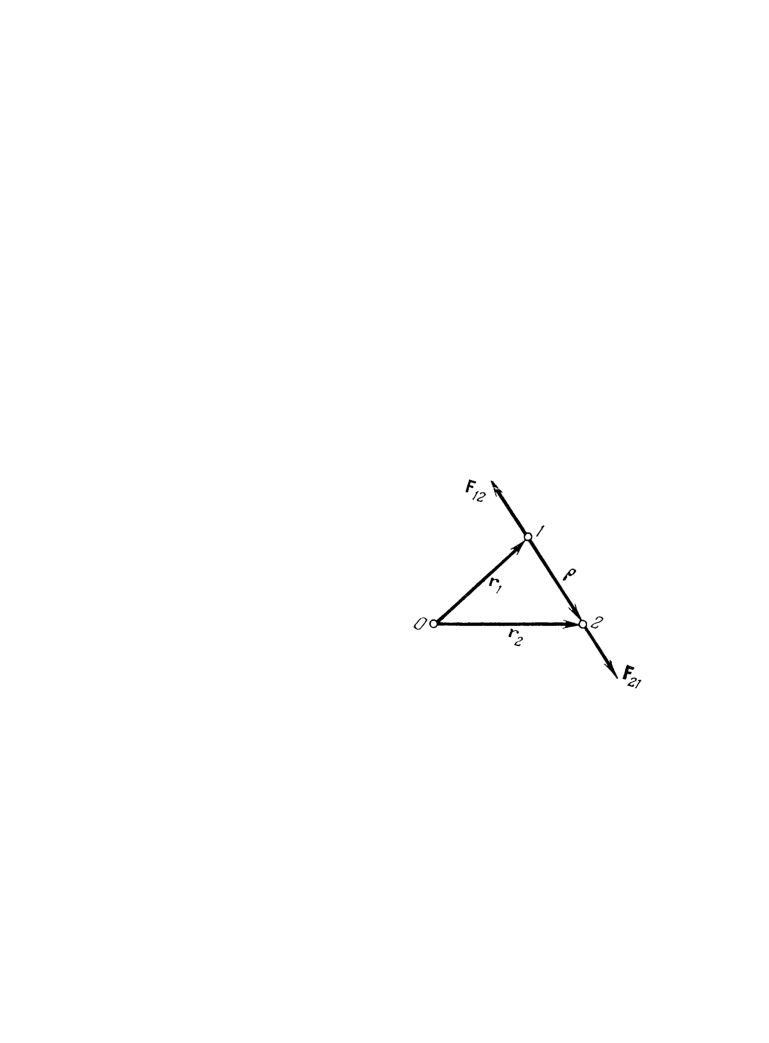
\includegraphics[width=0.8\textwidth]{figs/ch-03/fig-03-03.pdf}
%\input{figs/ch-03/fig-03-01}
%  \vspace{-13pt}
\sidecaption{Potential energy of a system of two particles with central forces.\zhcap{中心力作用下两质点系统的势能。}\label{fig-03-03}}
\end{marginfigure}

\subsection{}\label{3.3.5} \hlblue{Example~3.}  \redem{Potential energy of a system of two particles between which central forces} act, i.e. forces depending upon the distance between the particles and directed along the straight line joining the particles. Shown in \figr{fig-03-03} are mutually repul­sive forces $\vb{F}_{12}$ and $\vb{F}_{21}  = - \vb{F}_{12}$:
\zhpar{\hlblue{例3。}\redem{两质点之间作用有中心力时系统的势能。}即力仅依赖于两质点之间的距离，并沿连接两质点的直线方向。\figr{fig-03-03} 所示为相互排斥的力 $\vb{F}_{12}$ 与 $\vb{F}_{21}  = - \vb{F}_{12}$，如下所示。}
\begin{equation*}%
\vb{F}_{21} = F_{\rho} (\rho) \frac{\pmb{\rho}}{\rho},
\end{equation*}
where $\pmb{\rho} = \vb{r}_{2} - \vb{r}_{1}$ is the radius vector from particle 1 to par­ticle 2, and $F_{\rho} (\rho)$ is the projection of force $\vb{F}_{21}$ on the direction of vector $\pmb{\rho}$ and depends only on the distance $\rho$ between the particles. An infinitely small change in the potential energy of the system
\zhpar{式中 $\pmb{\rho} = \vb{r}_{2} - \vb{r}_{1}$ 为从质点 1 指向质点 2 的位矢，$F_{\rho} (\rho)$ 为力 $\vb{F}_{21}$ 在矢量 $\pmb{\rho}$ 方向上的投影，它仅依赖于两质点间的距离 $\rho$。系统势能的无限小改变量如下式所示。}
\begin{equation*}%
\dd E_{p} = -(\vb{F}_{12} \dd \vb{r}_{1} + \vb{F}_{21} \dd \vb{r}_{2}) 
= - \vb{F}_{21} \dd \pmb{\rho} = - F_{\rho} (\rho) \dd \rho.
\end{equation*}
If we assume that $E_{p} \to 0$ as $\rho \to \infty$, then
\zhpar{若假定当 $\rho \to \infty$ 时 $E_{p} \to 0$，则有如下关系式。}
\begin{equation*}%
E_{p} (\rho)=  \int_{\rho}^{\infty} F_{\rho} (\rho) \dd \rho.
\end{equation*}
This energy is often called the \redem{mutual po­tential energy of two particles.}
\zhpar{该能量通常称为\redem{两质点的相互势能}。}

\begin{marginfigure}[-2cm]
%\begin{wrapfigure}{r}{0.5\linewidth}
\centering
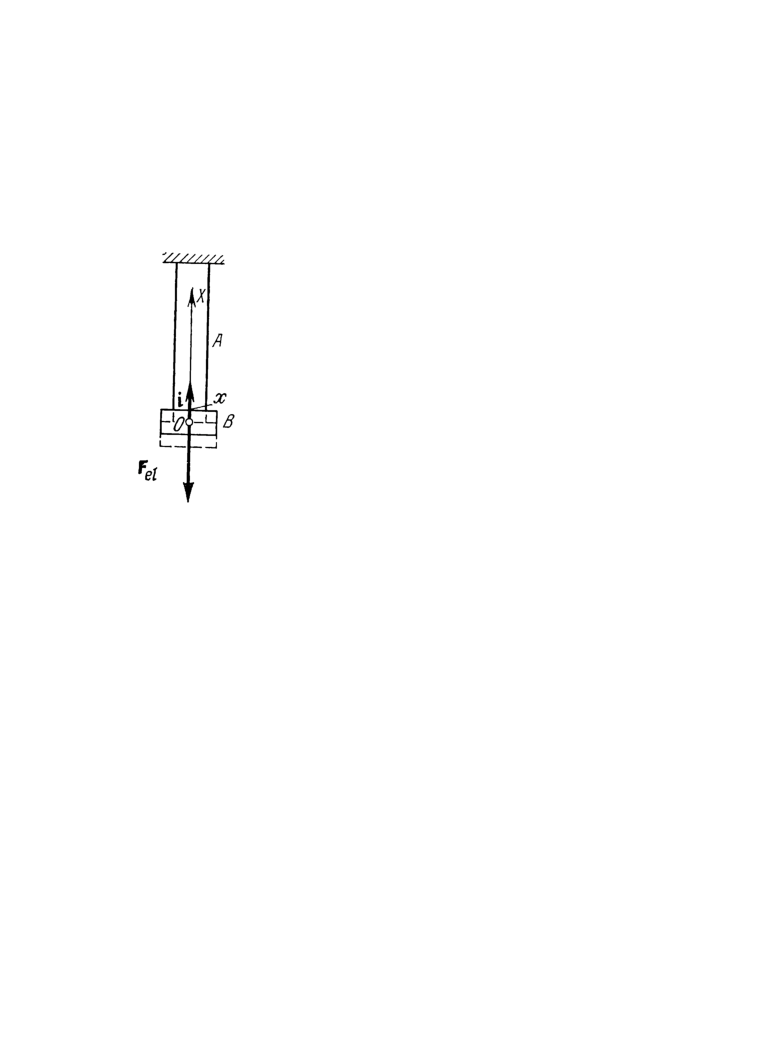
\includegraphics[width=0.4\textwidth]{figs/ch-03/fig-03-04.pdf}
%\input{figs/ch-03/fig-03-01}
%  \vspace{-13pt}
\caption{Potential energy of an elastic body in axial tension or compression. \zhcap{轴向拉伸或压缩时弹性体的势能。}\label{fig-03-04}}
\end{marginfigure}
\subsection{}\label{3.3.6} \hlblue{Example~4.} \redem{Potential energy of an elastic body (for instance, a spring) in axial tension or compression.} When an elastic body is deformed, conservative internal forces (elastic forces) are developed in the body that oppose deformation. According to Hooke's law, the force $\vb{F}_{\textrm{el}}$ exerted by the deformed body $A$ (\figr{fig-03-04}) on body $B$, causing the deformation, is proportional to the amount of deformation (stretch or compression):
\zhpar{\hlblue{例4。}\redem{承受轴向拉伸或压缩的弹性体（例如弹簧）的势能。}当弹性体发生形变时，体内会产生阻碍形变的保守内力（弹性力）。根据胡克定律，形变物体 $A$（见 \figr{fig-03-04}）作用于使其产生形变的物体 $B$ 上的弹性力 $\vb{F}_{\textrm{el}}$ 与形变量（伸长或压缩量）成正比，如下式所示。}
\begin{equation*}%
\vb{F}_{\textrm{el}} = - kx \vu{i}.
\end{equation*}
Here $x_{i}$ is the displacement vector of body $B$ that characterizes the deformation of body $A$ (in the undeformed state $x = 0$; in compression $x> 0$ and intension $x < 0$),and $k> 0$ is a factor characterizing the elastic properties of body $A$.
\zhpar{式中 $x_{i}$ 为物体 $B$ 的位移矢量，它表征物体 $A$ 的形变（未形变时 $x = 0$；压缩时 $x> 0$，拉伸时 $x < 0$），$k> 0$ 为表征物体 $A$ 弹性性质的系数。}

The potential energy of an elastically deformed body (in the absence of deformation, i.e. at $x = 0$, this energy is assumed equal to zero)
\zhpar{弹性形变物体的势能如下式所示（在无形变即 $x = 0$ 时，该能量取为零）。}
\begin{equation*}%
E_{p} = \frac{kx^{2}}{2}.
\end{equation*}

\section{Law of Conservation of Mechanical Energy}
\label{sec-3.4}
\zhtitle{机械能守恒定律}

\subsection{}\label{3.4.1} The \redem{mechanical energy}, or \redem{total mechanical energy}, is the energy of mechanical motion and interaction. The mechanical energy $E$ of a system of particles is equal to the sum of their kinetic energy $E_{k}$ and the potential energy $E_{p}$ of interaction of these particles with one another and with external bodies:
\zhpar{\redem{机械能}，或称\redem{总机械能}，是机械运动和相互作用的能量。质点系的机械能 $E$ 等于其动能 $E_{k}$ 与这些质点彼此之间以及与外部物体相互作用的势能 $E_{p}$ 之和，即如下式所示。}
\begin{equation*}%
E = E_{k} + E_{p}.
\end{equation*}
An elementary increment of the mechanical energy of a system during the infinitely short time $\dd t$ is equal to
\zhpar{系统在无限短时间 $\dd t$ 内机械能的无限小增量如下式所示。}
\begin{equation*}%
\dd E = \delta W_{\textrm{nonc}} + \pdv{E_{p}}{t} \dd t,
\end{equation*}
where $\delta W_{\textrm{nonc}}$ is the algebraic sum of the elements of work done in the time interval $\dd t$ by all the internal and external \redem{nonconservative} forces. The term $( \pdv*{E_{p}}{t}) \dd t$ represents the change during the time interval $\dd t$ in the potential energy of the system and, consequently, its total mechanical energy due to nonstationary external conservative forces \ssect{3.3.1}. 
\zhpar{式中 $\delta W_{\textrm{nonc}}$ 为在时间间隔 $\dd t$ 内所有内力与外力中\redem{非保守力}所做元功的代数和。项 $( \pdv*{E_{p}}{t}) \dd t$ 表示在时间间隔 $\dd t$ 内，由于外部非稳定保守力（见 \ssect{3.3.1}）而引起的系统势能的改变量，因而也就是系统总机械能的改变量。}

\subsection{}\label{3.4.2} If the system is \redem{conservative} \ssect{3.1.7}, $\delta W_{\textrm{nonc}} \equiv 0$ and $\pdv*{E_{p}}{t} = 0$, because, in this case, there are no nonconservative forces and the external conservative forces are stationary. Con­sequently, the mechanical energy of such a system $E = \textrm{const}$, i.e. the following law, called the \redem{law of conservation of mechan­ical energy}, is valid: in the motion of a conservative system, its mechanical energy remains unchanged.
\zhpar{若系统为\redem{保守系统}（见 \ssect{3.1.7}），则 $\delta W_{\textrm{nonc}} \equiv 0$ 且 $\pdv*{E_{p}}{t} = 0$，因为在这种情形下不存在非保守力，并且外部保守力是稳定的。因此，该系统的机械能 $E = \textrm{const}$，即成立\redem{机械能守恒定律}：保守系统运动时，其机械能保持不变。}

In particular, this law holds for closed conservative systems: the mechanical energy of a closed system does not change with time if all the internal forces acting in this system are conser­vative ones.
\zhpar{特别地，该定律对封闭保守系统同样成立：若系统中所有内力均为保守力，则封闭系统的机械能不随时间改变。}

The law of conservation of mechanical energy is associated with the \redem{uniformity of time}. This property of time is manifested in the fact that the laws of motion of a closed system (or a system located in a stationary external field) are independent of the choice of the zero time reference. For example, in the free fall of a body in a stationary conservative gravity field at the earth's surface, the velocity of the body and the length of path travelled depend only on the length of time in free fall and initial vel­ocity of the body, but not on the specific instant of time the body began to fall.
\zhpar{机械能守恒定律与\redem{时间的均匀性}相联系。时间的这一性质表现为：封闭系统（或位于稳定外场中的系统）的运动规律与零时刻的选取无关。例如，地球表面稳定保守重力场中物体的自由下落，其速度和所经路程长度仅取决于下落的时间长度和物体的初速度，而与物体开始下落的具体时刻无关。}

\subsection{}\label{3.4.3} The mechanical energy of a closed nonconservative system is changed owing to the work done by all the nonconservative internal forces:
\zhpar{封闭非保守系统的机械能，因其内部所有非保守内力做功而发生改变，即如下式所示。}
\begin{equation*}%
\dd E = \delta W_{\textrm{nonc}}.
\end{equation*}
Gyroscopic forces \ssect{3.1.7} do no work and make no contribution to $\delta W_{\textrm{nonc}}$, i.e. the existence of such forces in a system does not lead to changes in its mechanical energy.
\zhpar{陀螺力（见 \ssect{3.1.7}）不做功，对 $\delta W_{\textrm{nonc}}$ 没有贡献，即系统中存在此类力并不会导致其机械能发生改变。}

The action of dissipative forces \ssect{3.1.7}, for instance, the force of friction, leads to a gradual reduction in the mechanical energy of a closed system. This process is called the \redem{dissipation of energy}. Consequently, a system whose mechanical energy contin­ually decreases with time is called a \redem{dissipative system}. In the dissipation of energy, the mechanical energy of the system is converted into other forms of energy (for example, into the energy of chaotic motion of molecules). The conversion of mechanical energy is accomplished in full agreement with a universal law of nature: the law of conservation of energy \ssect{9.2.7}.
\zhpar{耗散力（见 \ssect{3.1.7}），例如摩擦力，会使封闭系统的机械能逐渐减少。这一过程称为\redem{能量耗散}。因此，机械能随时间不断减少的系统称为\redem{耗散系统}。在能量耗散过程中，系统的机械能转化为其他形式的能量（例如分子无规则运动的能量）。这种机械能的转化完全符合自然界的一条普遍规律——能量守恒定律（见 \ssect{9.2.7}）。}

According to this law, energy can be converted from one form to another and redistributed within the system, but its total amount in a closed system must remain constant. It follows from the law of conservation and conversion of energy that the changes in energy of an open system, occurring in interaction of the system with the external medium (external bodies and fields), must be numerically equal and opposite in sign to the changes in the energy of the external medium. In other words, the change in the energy of a system upon its interaction with the external medium should be equal to the energy the system receives or yields up in the process being considered.
\zhpar{根据这一定律，能量可以从一种形式转化为另一种形式，并在系统内部重新分布，但封闭系统中能量的总量必须保持不变。由能量守恒与转化定律可知，开放系统与外部介质（外部物体与场）相互作用时发生的能量变化，在数值上必与外部介质能量的变化相等、符号相反。换言之，系统与外部介质相互作用时的能量改变量，应等于系统在所考虑过程中从外界获得或输出的能量。}

\subsection{}\label{3.4.4} Forces of resistance and friction act in all real mechanical systems. Hence, these systems are nonconservative. In certain cases, however, they can be assumed approximately conserva­tive, and the law of conservation of mechanical energy can be applied to them. Such an approach is feasible if, in the process being considered, the work $W_{\textrm{nonc}}$ done by all the nonconserva­tive forces acting on the system is negligibly small in compari­son to the mechanical energy $E$ of the system, i.e. $\abs{W_{\textrm{nonc}}/E} \ll 1$, so that $\abs{\Delta E/E} \ll 1$, where $\Delta E = W_{\textrm{nonc}}$ is the change in the mechanical energy of the system.
\zhpar{一切实际的力学系统中都存在阻力与摩擦力，因此这些系统都是非保守的。然而，在某些情形下，它们可以近似地视为保守的，此时可以应用机械能守恒定律。这种处理方法是可行的，前提是所考虑的过程中，作用于系统的所有非保守力所做的功 $W_{\textrm{nonc}}$ 与系统的机械能 $E$ 相比可以忽略不计，即 $\abs{W_{\textrm{nonc}}/E} \ll 1$，从而 $\abs{\Delta E/E} \ll 1$，其中 $\Delta E = W_{\textrm{nonc}}$ 为系统机械能的改变量。}

\subsection{}\label{3.4.5} The state of \redem{mechanical equilibrium of a system} is one that can be disturbed only as a result of external force action applied to the system. In this equilibrium state all the particles of the system are at rest so that the kinetic energy of the system equals zero. The state of mechanical equilibrium is said to be \redem{stable} if a small external action applied to the system leads to only a small change in its state. In this case, forces are devel­oped in the system that tend to restore the equilibrium state. A state of mechanical equilibrium is said to be \redem{unstable} if it can be disturbed by even an infinitely small external action on the system, which does not return again to the equilibrium state. In this case, forces are developed in the system that tend to further disturb the equilibrium state.
\zhpar{\redem{系统的力学平衡}状态是指只能通过对系统施加外力作用而被扰动的状态。在这种平衡状态下，系统中所有质点都处于静止，因而系统动能为零。若对系统施加微小的外部作用只会引起其状态的微小改变，则称该力学平衡状态为\redem{稳定}的；此时系统中会产生趋于恢复平衡状态的力。若平衡状态即使受到无限小的外部作用就会被扰动，并且系统不会自行回到平衡状态，则称该力学平衡状态为\redem{不稳定}的；此时系统中会产生进一步扰动平衡状态的力。}

The law of conservation of mechanical energy enables the condi­tions of equilibrium of conservative systems to be formulated:
\zhpar{机械能守恒定律使得保守系统的平衡条件可以表述如下。}

in states of stable equilibrium the potential energy curve of the system has minima, whereas in states of unstable equilib­rium, it has maxima.
\zhpar{处于稳定平衡状态时，系统的势能曲线具有极小值；而处于不稳定平衡状态时，势能曲线具有极大值。}

\subsection{}\label{3.4.6} On the basis of the law of conservation of mechanical energy, the region of possible configurations of a conservative system \ssect{3.3.1} can be found. The kinetic energy of the system $E_{k} \gg 0$. Hence, at a given value $E$ of the mechanical energy of the system, the latter can only be in states that conform to the condition: $E_{p} \ll E$. \figr{fig-03-05} illustrates the simplest case in which a particle has one-dimensional motion along axis OX in an external stationary conservative field. The potential energy of the particle is a function of only a single coordinate $x$, i.e. $E_{p} = E_{p} (x)$. The curve of this relation, shown in \figr{fig-03-05}, is called a \redem{potential energy curve}. 
\zhpar{依据机械能守恒定律，可以求出保守系统（见 \ssect{3.3.1}）可能的位形区域。系统的动能 $E_{k} \gg 0$。因此，在给定系统机械能 $E$ 的值时，系统只能处于满足条件 $E_{p} \ll E$ 的状态。\figr{fig-03-05} 所示为最简单的情形：质点在外部稳定保守场中沿 OX 轴作一维运动。质点的势能仅是单一坐标 $x$ 的函数，即 $E_{p} = E_{p} (x)$。该函数关系的曲线（见 \figr{fig-03-05}）称为\redem{势能曲线}。}
\begin{figure}%[!ht]
%\begin{wrapfigure}{r}{0.5\linewidth}
\centering
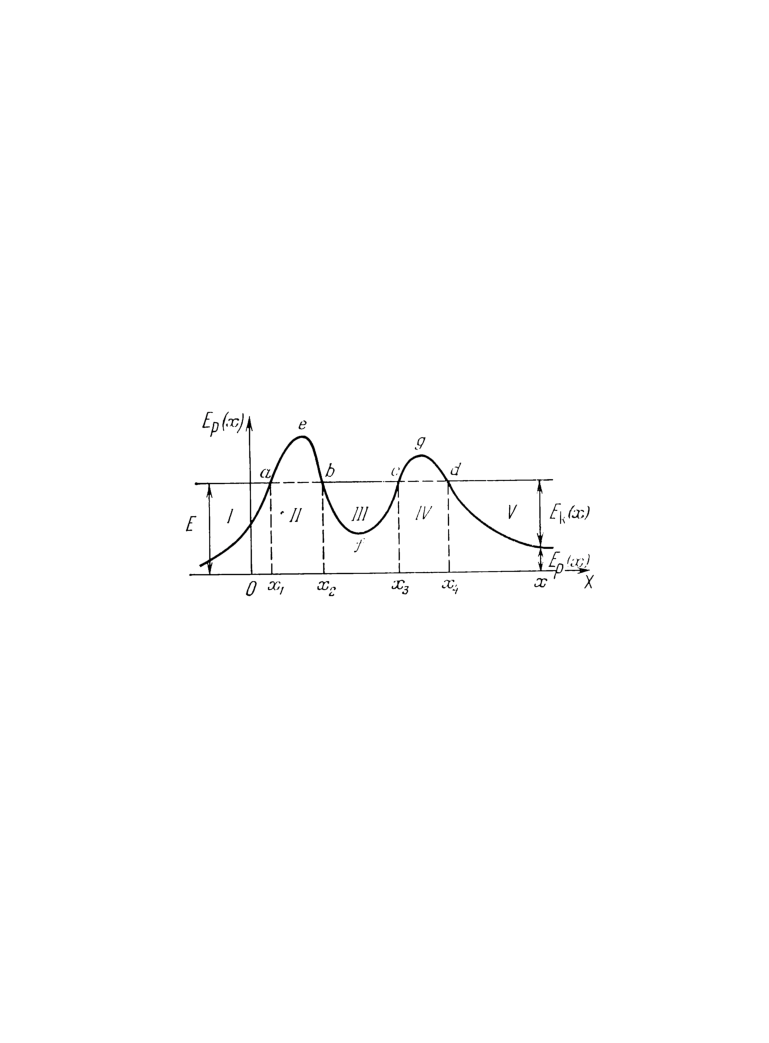
\includegraphics[width=0.9\textwidth,angle=-1]{figs/ch-03/fig-03-05.pdf}
%\input{figs/ch-03/fig-03-01}
%  \vspace{-13pt}
\sidecaption{Potential energy curve for the motion of a particle in an external stationary conservative field.\zhcap{质点在外部稳定保守场中运动的势能曲线。}
\label{fig-03-05}}
\end{figure}


For a fixed value of the mechanical energy $E$ of the particle, as shown in \figr{fig-03-05}, the particle can remain, in its travel, in one of the following three regions: 
\zhpar{对于质点给定的机械能 $E$，如 \figr{fig-03-05} 所示，质点在运动过程中可处于以下三个区域之一，即如下式所示。}
\begin{align*}%
x & \leqslant x_{1} \,\, \textrm{(region I)},\\
x_{2} & \leqslant x \leqslant x_{3}\,\, \textrm{(region III)}, \qand \\
x & \geqslant x_{4}\,\, \textrm{(region V)}.
\end{align*}
These regions are separated from one another by the regions II and IV, which are the so-called \redem{potential barriers} $aeb$ and $cgd$, within whose limits the particle cannot exist. At the boundaries of the potential barriers (at points $a,\, b,\, c$ and $d$), the particle reverses its direction of motion; in region I the particle can travel without limit to the left of boundary $a$ of the barrier, and in region V, without limit to the right of bound­ary $d$ of the barrier. In region III, the particle oscillates be­tween points $b$ and $c$; it is in a so-called \redem{potential well} $bfc$.
\zhpar{这些区域被区域 II 与区域 IV 隔开，区域 II 与区域 IV 即所谓的\redem{势垒} $aeb$ 与 $cgd$，质点不能存在于其范围之内。在势垒边界（$a$、$b$、$c$、$d$ 各点）处，质点的运动方向发生反转：在区域 I 中，质点可以在势垒边界 $a$ 左侧无限制地运动；在区域 V 中，质点可以在势垒边界 $d$ 右侧无限制地运动。在区域 III 中，质点在 $b$ 与 $c$ 两点之间振荡，即处于所谓的\redem{势阱} $bfc$ 之中。}

\section{Perfectly Elastic and Inelastic Collisions}
\label{sec-3.5}
\zhtitle{完全弹性与非弹性碰撞}

\subsection{}\label{3.5.1} An impact in which a considerable change in the veloc­ities of the colliding bodies occurs in an extremely short time interval is called a \redem{collision}. Examples of collisions are a ham­ mer striking a billet being forged that lies on the anvil, and a hammer striking the head of a nail being driven.
\zhpar{在极短时间间隔内碰撞物体的速度发生显著改变的冲击称为\redem{碰撞}。例如，锤子敲击放在铁砧上待锻造的工件，或锤子敲打正在钉入的钉子头部，都是碰撞的例子。}

The \redem{line of impact} is the common normal to the surfaces of the colliding bodies at their point of contact. If the centres of mass \ssect{2.3.3} of the colliding bodies lie on the line of impact at the instant of contact, the collision is said to be \redem{central}. An example is the collision of two billiard balls. The collision, or impact, is said to be \redem{head-on}, or \redem{straight-line}, if the velocities of the centres of mass of the colliding bodies are parallel, before the collision, to the line of impact. Otherwise, it is called an \redem{oblique impact}, or \redem{glancing collision}.
\zhpar{\redem{碰撞线}是碰撞物体在接触点处表面的公法线。若在接触瞬间，两碰撞物体的质心都位于碰撞线上，则称该碰撞为\redem{对心碰撞}，例如两个台球的碰撞。若碰撞前两碰撞物体质心的速度都与碰撞线平行，则称该碰撞为\redem{正碰撞}（或\redem{直线碰撞}）；否则称为\redem{斜碰撞}（或\redem{擦碰撞}）。}

\subsection{}\label{3.5.2} In a collision the bodies are deformed and instantaneous, but quite substantial, forces are developed. They are called \redem{impact forces}. For a system of colliding bodies these forces are internal ones\sidenote{It is assumed that the colliding bodies are either free \ssect{2.2.3} or the constraints imposed on them are such that no impact constraint reactions are developed.}, i.e. they do not change the total momentum of the system. External forces, constantly exerted on the system (for instance, the gravity forces of the bodies) are usually very small compared to the impact forces. Therefore, even though the impulses of impact forces \ssect{2.4.2} in the duration $\tau$ of the collision are commensurable with the momenta \ssect{2.3.4} of the colliding bodies, the resultant impulse of all the constantly acting external forces during the same time interval $\tau$ is small compared to the momenta of the bodies. Accordingly, the work done on the system by the external forces during the time inter­ val t is small compared to the mechanical energy of the system. Hence, a system of bodies can be assumed, in the collision pro­ cess, to be an approximately closed system \ssect{2.2.4}. This means that in calculating the results of the collision, use can be made of the laws of the conservation of momentum \ssect{2.7.1}, of angular momentum \ssect{4.4.1} and of energy \ssect{9.2.7}. If the bodies deform in the collision like perfectly elastic ones, the impact forces are conservative and the law of conservation of mechanical energy \ssect{3.4.2} is valid in the system.
\zhpar{碰撞中物体发生形变，并产生瞬时但相当大的力，称为\redem{冲击力}。对于碰撞物体组成的系统，这些力是内力，因此它们不改变系统的总动量。作用于系统上的外力（例如物体的重力）通常远小于冲击力。因此，尽管在碰撞持续时间 $\tau$ 内冲击力的冲量（见 \ssect{2.4.2}）与碰撞物体的动量（见 \ssect{2.3.4}）可以比拟，但在同一时间间隔 $t$ 内所有持续作用的外力的合冲量相对于物体的动量仍然很小。相应地，在时间间隔 $t$ 内外力对系统所做的功也远小于系统的机械能。因此，在碰撞过程中，物体系统可以近似地视为封闭系统（见 \ssect{2.2.4}）。这意味着，在计算碰撞结果时，可以应用动量守恒定律（见 \ssect{2.7.1}）、角动量守恒定律（见 \ssect{4.4.1}）以及能量守恒定律（见 \ssect{9.2.7}）。若物体在碰撞中像完全弹性体那样发生形变，则冲击力为保守力，系统中机械能守恒定律（见 \ssect{3.4.2}）成立。}
\zhpar{注：假定碰撞物体是自由的（见 \ssect{2.2.3}），或者对其施加的约束使得碰撞中不产生冲击约束反力。}

\subsection{}\label{3.5.3} The collision of two bodies is said to be \redem{perfectly inelastic} if, after impact, they travel together as a single body. Suffi­ciently close to a perfectly inelastic collision are, for example, the impact of the pile-driving hammer with the end of the pile being driven, and the firing of a bullet into a wagon filled with sand, when the bullet remains embedded in the sand. Various processes occur in the colliding bodies in an inelastic collision (plastic deformation of the bodies, friction, etc.). As a result, the kinetic energy of the system is partly transformed into its internal energy \ssect{9.1.2}.
\zhpar{若两物体在碰撞后以一个整体一起运动，则称两物体的碰撞为\redem{完全非弹性碰撞}。例如，打桩锤撞击待打入桩的顶端，或子弹射入装满沙子的车厢并留在沙中，都与完全非弹性碰撞十分接近。非弹性碰撞中，碰撞物体内部会发生各种过程（物体的塑性形变、摩擦等）。结果，系统的动能部分地转化为其内能（见 \ssect{9.1.2}）。}

If.two bodies of masses $m_{1}$ and $m_{2}$, travelling with translational motion at the velocities $\vb{v}_{1}$ and $\vb{v}_{2}$, undergo a \redem{perfectly inelastic head-on central collision}, they continue their translational motion together at the velocity
\zhpar{若质量分别为 $m_{1}$ 和 $m_{2}$、速度分别为 $\vb{v}_{1}$ 和 $\vb{v}_{2}$ 并作平动的两物体发生\redem{完全非弹性正碰撞}（对心碰撞），则碰撞后它们以如下速度一起作平动。}
\begin{equation*}%
\vb{u} = \frac{m_{1}\vb{v}_{1}+ m_{2}\vb{v}_{2}}{m_{1}+m_{2}}.
\end{equation*}
\hlblue{Note.} In the case of a perfectly inelastic collision that is neither head-on nor central, the preceding equation can be used to find the velocity of the centre of the mass of the bodies joined to­gether in the collision. As the result of such a collision, how­ ever, the system may begin to rotate about its centre of mass in accordance with the law of conservation of angular momen­tum \ssect{4.4.1}.
\zhpar{\hlblue{注意。}对于既非正碰撞也非对心碰撞的完全非弹性碰撞，上式可用来求碰撞后结合在一起的物体的质心速度。然而，由于这种碰撞，系统可能依据角动量守恒定律（见 \ssect{4.4.1}）绕其质心转动。}

\subsection{}\label{3.5.4} The change in the kinetic energy of a system of two collid­ing bodies in a perfectly inelastic head-on central collision is
\zhpar{在完全非弹性正碰撞中，两碰撞物体组成的系统动能的改变量如下式所示。}
\begin{align*}%
\Delta E_{k} & = \frac{m_{1}+ m_{2}}{2} \vb{u}^{2} -  \frac{m_{1}}{2} \vb{v}^{2}_{1}-  \frac{m_{2}}{2} \vb{v}^{2}_{2}, \\
& = -\frac{m_{1}m_{2}}{2(m_{1}+m_{2})} (\vb{v}_{1}^{2} -\vb{v}_{2}^{2} ) < 0.
\end{align*}
In particular, if the second, body is at rest before the collision (for instance, a pile being driven by a pile driver, or a forging lying on the anvil), the relative reduction in the kinetic energy of the system in a perfectly inelastic head-on central collision is
\zhpar{特别地，若碰撞前第二个物体静止（例如被打桩机打入的桩，或放在铁砧上的锻件），则在完全非弹性正碰撞中，系统动能的相对减少量如下式所示。}
\begin{equation*}%
- \frac{\Delta E_{k}}{E_{k_{1}}} = \frac{ m_{2}}{m_{1}+m_{2}}.
\end{equation*}
In engineering, a perfectly inelastic head-on central collision (impact) is made use of to change the shape of bodies (smith and die forging, rivetting, etc.) or to move a body in a medium with high resistance to motion (driving nails, piles, etc.). It proves expedient in the first case to have the ratio $-\Delta E_{k}/E_{k_{1}}$ as near as possible to unity, i.e. it is necessary that $m_{2} \gg m_{1}$ (the mass of the forged item and the anvil should be many times greater than that of the hammer). In the second case, on the contrary, it is necessary that the loss in kinetic energy in the collision (impact) be as low as possible, i.e. that $m_{1} \gg m_{2}$ (the mass of the hammer should be many times greater than that of the nail being driven).
\zhpar{在工程中，利用完全非弹性正碰撞（冲击）来改变物体的形状（如锻造、模锻、铆接等），或使物体在阻力很大的介质中运动（如打入钉子、桩等）。在第一种情形中，希望比值 $-\Delta E_{k}/E_{k_{1}}$ 尽可能接近于 1，即要求 $m_{2} \gg m_{1}$（锻件与铁砧的质量应远大于锤子的质量）。而在第二种情形中则恰恰相反，要求碰撞（冲击）中动能损失尽可能小，即 $m_{1} \gg m_{2}$（锤子的质量应远大于被打入钉子的质量）。}

\subsection{}\label{3.5.5}A collision is said to be \redem{perfectly elastic} if it does not lead to any change in the mechanical energy of the system, i.e. if the bodies are perfectly elastic.
\zhpar{若碰撞不引起系统机械能的任何改变，即物体是完全弹性的，则称该碰撞为\redem{完全弹性碰撞}。}

\hlblue{Example 1.} A perfectly elastic head-on central collision of two bodies (for instance, balls) of masses $m_{1}$ and $m_{2}$, which travel before the collision with translational motion at the velocities $\vb{v}_{1}$ and $\vb{v}_{2}$ along axis $OX$, passing through their centres of mass (\figr{fig-03-06}~\textcolor{IndianRed}{(a)}). The velocities of the bodies after the collision, $\vb{u}_{1}$ and $\vb{u}_{2}$ (\figr{fig-03-06}~\textcolor{IndianRed}{(b)}), can be found from the laws of conserva­tion of momentum and mechanical energy:
\zhpar{\hlblue{例1。}质量分别为 $m_{1}$ 和 $m_{2}$ 的两物体（例如小球）发生完全弹性正碰撞。碰撞前，两物体沿 OX 轴作平动，速度分别为 $\vb{v}_{1}$ 和 $\vb{v}_{2}$，且速度方向通过各自的质心（见 \figr{fig-03-06}~\textcolor{IndianRed}{(a)}）。碰撞后两物体的速度 $\vb{u}_{1}$ 与 $\vb{u}_{2}$（见 \figr{fig-03-06}~\textcolor{IndianRed}{(b)}）可由动量守恒定律与机械能守恒定律求得，如下式所示。}
\begin{align*}%
m_{1}\vb{u}_{1} + m_{2}\vb{u}_{2} & = m_{1}\vb{v}_{1} + m_{2}\vb{v}_{2},\\
m_{1}\vb{u}_{1}^{2} + m_{2}\vb{u}_{2}^{2} & = m_{1}\vb{v}_{1}^{2} + m_{2}\vb{v}_{2}^{2}.\\
\end{align*}
\begin{figure}%[!ht]
%\begin{wrapfigure}{r}{0.5\linewidth}
\centering
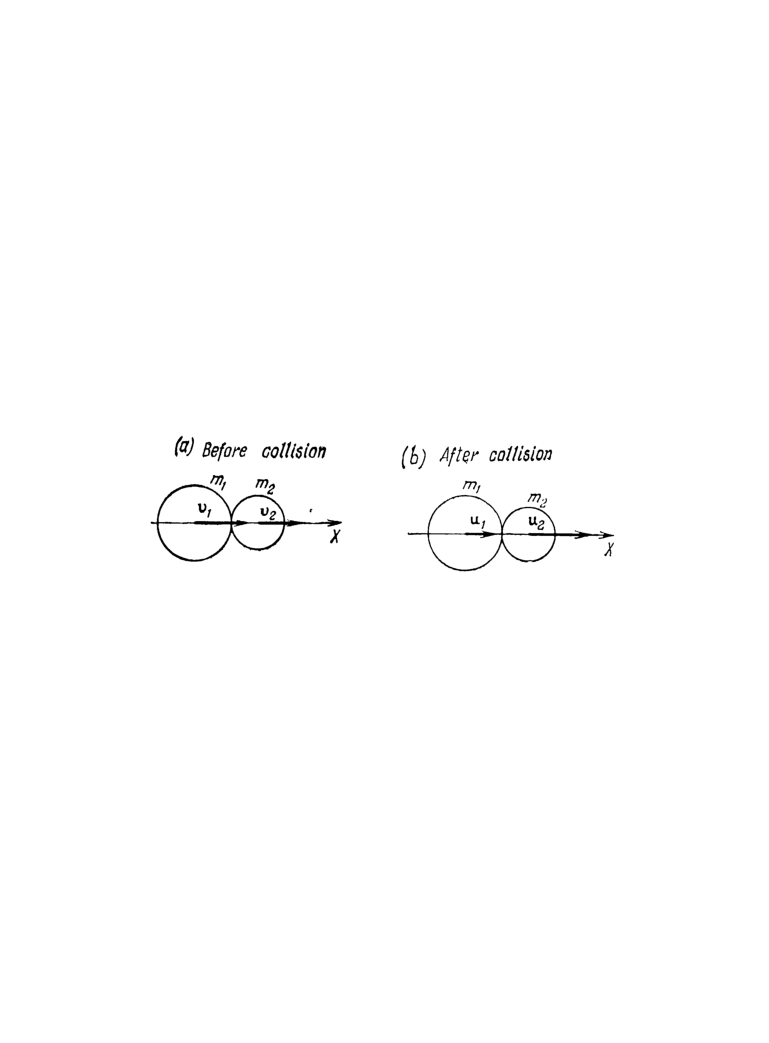
\includegraphics[width=0.8\textwidth,angle=-1]{figs/ch-03/fig-03-06.pdf}
%\input{figs/ch-03/fig-03-01}
%  \vspace{-13pt}
\sidecaption{A perfectly elastic head-on central collision of two bodies.\zhcap{两物体的完全弹性正碰撞。}\label{fig-03-06}}
\end{figure}

Velocities $\vb{u}_{1}$ and $\vb{u}_{2}$ are directed along axis $OX$ and their projections on this axis are
\zhpar{速度 $\vb{u}_{1}$ 与 $\vb{u}_{2}$ 沿 OX 轴方向，它们在该轴上的投影如下式所示。}
\begin{equation*}%
u_{1x} = \frac{(m_{1} - m_{2})v_{1x} + 2m_{2}v_{2x}}{m_{1}+m_{2}}
\end{equation*}
and
\zhpar{和}
\begin{equation*}%
u_{2x} = \frac{2m_{1}v_{1x} + (m_{2} - m_{1})v_{2x}}{m_{1}+m_{2}}
\end{equation*}
In particular, if the masses of the bodies are the same, the bodies exchange velocities in a collision: $u_{1x} = v_{2x}$ and $u_{2x} = v_{1x}$.
\zhpar{特别地，若两物体质量相同，则碰撞中二者交换速度，即 $u_{1x} = v_{2x}$，$u_{2x} = v_{1x}$。}

If the mass of the second body is many times greater than that of the first body, then $u_{1x} \approx 2v_{2x} - v_{1x}$ and $u_{2x} \approx v_{2x}$.
\zhpar{若第二个物体的质量远大于第一个物体的质量，则 $u_{1x} \approx 2v_{2x} - v_{1x}$，$u_{2x} \approx v_{2x}$。}

\subsection{}\label{3.5.6}  \hlblue{Example 2.} \redem{Perfectly elastic oblique central collision.} If the bodies are smooth the impulse of friction forces in the collision can be neglected. In this case the tangential compo­nents of the velocities of the bodies are not changed, i.e. compo­nents perpendicular to the line of impact: $u_{1} \tau = v_{1} \tau$ and $u_{2\tau} = v_{2\tau}$. The normal components, directed along the line of impact, change in the same way as in a head-on collision:
\zhpar{\hlblue{例2。}\redem{完全弹性斜碰撞。}若物体是光滑的，则碰撞中摩擦力的冲量可以忽略不计。此时，速度的切向分量（即垂直于碰撞线的分量）在碰撞中保持不变，即 $u_{1} \tau = v_{1} \tau$ 与 $u_{2\tau} = v_{2\tau}$。沿碰撞线方向的法向分量的变化与正碰撞相同，如下式所示。}
\begin{equation*}%
u_{1n} = \frac{(m_{1} - m_{2})v_{1n} + 2m_{2}v_{2n}}{m_{1}+m_{2}}
\end{equation*}
and
\zhpar{和}
\begin{equation*}%
u_{2n} = \frac{2m_{1}v_{1n} + (m_{2} - m_{1})v_{2n}}{m_{1}+m_{2}}
\end{equation*}
In particular, in the perfectly elastic oblique collision of a smooth ball with a fixed flat wall$(m_{2} \gg m_{1}$ and $u_{2}= v_{2}= 0)$:  $u_{1\tau} = v_{2\tau}$ and $u_{1n} = - v_{1n}$, i.e. the ball rebounds from the wall according to the law of mir­ror reflection: the angle of reflection is equal to the angle of incidence. The magnitude of the velocity is conserved: $u_{1}= v_{1}$. The vector $\Delta \vb{p}_{1}$ of the change in momentum of the ball in the collision is directed perpendicular to the wall:
\zhpar{特别地，在光滑小球与固定平面墙壁（$m_{2} \gg m_{1}$ 且 $u_{2}= v_{2}= 0$）的完全弹性斜碰撞中：$u_{1\tau} = v_{2\tau}$，$u_{1n} = - v_{1n}$，即小球按镜面反射定律从墙面弹回，反射角等于入射角。速度的大小保持不变：$u_{1}= v_{1}$。碰撞中小球动量的改变量 $\Delta \vb{p}_{1}$ 垂直于墙面，如下式所示。}
\begin{equation*}%
\Delta \vb{p}_{1} = m_{1}(\vb{u}_{1} -\vb{v}_{1}) = - 2m_{1}\vb{v}_{1n}
\end{equation*}
The impulse of impact force acting on the wall is equal to $2m_{1}\vb{v}_{1n}$.
\zhpar{作用于墙面的冲击力的冲量等于 $2m_{1}\vb{v}_{1n}$。}

%\begin{equation*}%
%\vb{F}= \sum_{i=1}^{n} \vb{F_{i}}
%\end{equation*}

%\end{wrapfigure}

%\begin{align*}%
%m\vb{a} = \vb{F}\,\,\textrm{and}\,\, \vb{F}_{ki} = - \vb{F}_{ik}\,\, \intertext{(in reference frame $K$)}\\
%m'\vb{a}' = \vb{F}'\,\,\textrm{and}\,\, \vb{F}_{ki}' = - \vb{F}_{ik}'\,\, \intertext{(in reference frame $K'$)}
%\end{align*}
